\باب{پس نوشت}\شناخت{باب_پس_نوشت}
%typing complete
 میں توقع کرتا ہوں کہ  آپ کوانٹائی میکانیات کو اب  سمجھتے ہوں گے لہٰذا   حصہ \حوالہ{حصہ_تفاعل_موج_شماریاتی_مفہوم} میں کیا گیا سوال دوبارہ اٹھاتے ہیں: کوانٹائی میکانیات کے نتائج سے کیا مطلب  اخذ  کرنا چاہیے؟ تفاعل موج کے ساتھ وابستہ شماریاتی مفہوم کی عدم تعیّنیت،  مسئلے کی  جڑ  ہے۔ تفاعل \عددی{\Psi}( یا کوانٹائی حال کہنا زیادہ  بہتر ہوگا؛  جو مثال کے طور پر،  چکرکار ہو سکتا ہے)      پیمائش کا نتیجہ یکتا طور پر تعین نہیں کرتا؛  بلکہ ممکنہ نتائج کی شماریاتی تقسیم مہیا کرتا ہے۔  اس سے ایک اہم سوال کھڑا ہوتا ہے: کیا پیمائش سے قبل نظام یہ مخصوص خاصیت \قول{ حقیقتاً رکھتا تھا}  ( جسے  \اصطلاح{حقیقت پسند}\فرہنگ{حقیقت پسند}\فرہنگ{realist} نقطہ نظر کہتے ہیں)  یا پیمائش کے عمل نے اس خاصیت کو \قول{ جنم}  دیا،  جو تفاعل موج کی شماریاتی پابندی کو مطمئن کرتا ہے (\اصطلاح{تقلید پسند }\فرہنگ{تقلید پسند}\فرہنگ{orthodox} نقطہ نظر)؛  یا ہم اس سوال کو ان بنیادوں پر رد کرتے ہیں کہ یہ  ایک فرضی سوال ہے  (\اصطلاح{انکاری}\فرہنگ{انکاری}\فرہنگ{agnostic} نقطہ نظر)؟

حقیقت پسند کے نقطہ نظر سے کوانٹائی میکانیات  \ترچھا{ نامکمل} نظریہ ہے،  چونکہ کوانٹائی میکانیات کی تمام فراہم کردہ معلومات ( یعنی اس کا تفاعل موج)  جانتے کے باوجود  آپ  اس کے خواص تعین نہیں کر سکتے ہیں۔ ظاہر ہے،  کوانٹائی میکانیات کے دائرہ کار  سے باہر،  مزید   معلومات  ہوگی  جو (\عددی{\Psi} کے ساتھ مل کر)   طبیعی حقائق  مکمل طور پر بیان کرے گی۔

تقلید پسند نقطہ نظر اس سے بھی زیادہ سنگین سوالات کھڑے کرتا ہے،  چونکہ اگر پیمائشی عمل نظام کو ایک ایسی  خاصیت اختیار کرنے پر مجبور کرتا ہو جو اس میں پہلے نہیں پائی جاتی تھی،\حاشیہد{میں یہاں کہنا چاہتا ہوں کہ،  مثلاً،اگر  ایک الیکٹران  چکری حال \عددی{\chi=\begin{psmallmatrix} 1\\0 \end{psmallmatrix}} میں ہو؛ اس کے زاویائی معیار حرکت کے \عددی{x} جزو کی پیمائش \عددی{\hslash/2} یا (برابر احتمال کے ساتھ) \عددی{-\hslash/2} دے سکتی ہے، تاہم پیمائش سے قبل \عددی{S_x} کی  پوری طرح معین قیمت نہیں  ہو گی۔}   تب پیمائش ایک عجیب عمل ہوگا۔ ساتھ ہی یہ جانتے ہوئے کہ ایک پیمائش کے فوراً بعد دوسری پیمائش وہی نتیجہ دیتی ہے،  ہمیں ماننا ہوگا کہ پیمائشی عمل تفاعل موج کو یوں\اصطلاح{ منہدم}\فرہنگ{منہدم}\حاشیہب{collapses}\فرہنگ{collapse}  کرتا ہے،  جو مساوات شروڈنگر کی تجویز کردہ ارتقا کے برعکس ہے۔ 

اس کی روشنی میں،  ہم دیکھ سکتے ہیں کہ نسل در نسل ماہر طبیعیات انکاری سوچ کے پیچھے پناہ  لینے پر کیوں  مجبور  ہوئے،  اور اپنے شاگردوں کو  نصیحت کرتے رہے کہ نظریے کی  تصوراتی بنیادوں پر غور و فکر کر کے اپنا وقت ضائع نہ کریں۔

\حصہ{آئنشٹائن، پوڈلسکی و روزن تضاد}
\سن{1935}میں آئنشٹائن،  پوڈلسکی اور روزن نے مل کر \اصطلاح{آئنشٹائن، پوڈلسکی و  روزن تضاد}\فرہنگ{آئنشٹائن، پوڈلسکی و روزن تضاد}\حاشیہب{EPR paradox}\فرہنگ{EPR paradox}  پیش کیا، جس کا مقصد (خالصتاً نظریاتی بنیادوں پر)  یہ ثابت کرنا تھا کہ صرف حقیقت پسندانہ  نقطہ نظر درست ہو سکتا ہے۔ میں آئنشٹائن، پوڈلسکی و  روزن  تضاد کا  ایک سادہ روپ،  جو  داؤد بوہم نے  متعارف کیا،  پر تبصرہ کرتا ہوں۔ تعدیلی  \اصطلاح{پائے میزون}\فرہنگ{میزون!پائے}\حاشیہب{pi meson}\فرہنگ{meson!pi}  کی ایک الیکٹران اور ایک پروٹان میں  تنزل:
\begin{align*}
	\pi^0\to e^{-}+e^{+}
\end{align*}
 پر غور کریں۔
\begin{figure}
\centering
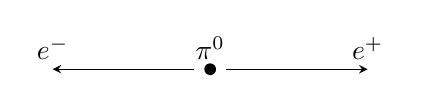
\begin{tikzpicture}
\draw[-stealth] (-0.2,0) -- (-2,0) node[above]{$e^{-}$};
\draw[-stealth] (0.2,0) -- (2,0) node[above]{$e^{+}$};
\draw[] (0,0) node[circle, inner sep=1.5pt, fill=black]{} node[above]{$\pi^{0}$};
\end{tikzpicture}
\caption{آئنشٹائن، پوڈلسکی و  روزن  تضاد کا بوہم انداز۔ساکن \عددی{\pi^0}  کا تنزل الیکٹران اور   ضد الیکٹران  جوڑی میں ہوتا ہے۔}
\label{شکل_بکھراو_بوہم_تنزل}
\end{figure}
%
ساکن پایون کی صورت میں الیکٹران اور پروٹان ایک دوسرے کے مخالف رخ جائیں گے (شکل \حوالہ{شکل_بکھراو_بوہم_تنزل})۔   پایون کا چکر صفر ہے،  لہٰذا زاویائی معیار حرکت کے  بقا کے تحت یہ الیکٹران اور ضد الیکٹران  یک تا تشکیل:
\begin{align}\label{مساوات_پس_ہمبستہ}
	\frac{1}{\sqrt{2}}(\uparrow_{-}\downarrow_{+}-\downarrow_{-}\uparrow_{+})
\end{align}
  میں ہوں گے۔ اگر  الیکٹران ہم میدان میں پایا جائے،  تو  ضد الیکٹران لازماً خلاف میدان ہوگا،   اور اسی طرح اگر الیکٹران خلاف میدان پایا جائے تو ضد الیکٹران ہم میدان ہوگا۔ کوانٹائی میکانیات آپ کو یہ بتانے سے قاصر ہے کہ کسی ایک  پایون تحویل میں آپ کو کونسی جوڑی   ملے گا،  لیکن کوانٹائی میکانیات یہ ضرور بتا سکتی ہے کہ ان پیمائش کا ایک دوسرے کے ساتھ \اصطلاح{باہمی رشتہ}\فرہنگ{باہمی رشتہ}\حاشیہب{correlated}\فرہنگ{correlated}  ہوگا،  اور  (اوسطاً)  نصف وقت ایک قسم اور نصف وقت دوسری قسم کی جوڑیاں پیدا ہوں گے۔ اب فرض کریں،  ہم ان الیکٹران اور ضد الیکٹران کو دور جانے دیں؛   عملی تجربے  میں  دس میٹر دور، یا،  اصولی تجربہ میں دس نوری سال  دور؛  اور اس کے بعد الیکٹران کے چکر کی پیمائش کریں۔ فرض کریں آپ کو ہم میدان ملتا ہے۔ آپ فوراً جان پائیں گے کہ بیس میٹر  (یا بیس نوری سال)  دور  دوسرے  شخص کو   ضد الیکٹران  خلاف میدان ملے  گا، اگر وہ  اس ضد الیکٹران پر پیمائش کرے ۔
  
\قول{حقیقت پسند}  نقطہ نظر سے اس میں کوئی حیرانی کی بات نہیں؛  پیدائش کے وقت سے ہی الیکٹران حقیقتاً ہم میدان  اور ضد الیکٹران خلاف میدان تھے؛   ہاں کوانٹائی میکانیات اس  بارے میں جاننے سے قاصر تھی۔ تاہم ، \قول{تقلید پسند}  نقطہ نظر کے تحت پیمائش سے قبل دونوں ذرات نہ ہم میدان اور نہ ہی خلاف میدان تھے؛  الیکٹران پر پیمائش تفاعل موج کو منہدم کرتی ہے جو  بیس میٹر (یا بیس نوری سال)  دور ضد الیکٹران کو فوراً  خلاف میدان  \قول{بناتی} ہے۔ آئنشٹائن،  پوڈلسکی اور روزن اس قسم کے فاصلاتی  عمل کرنے والے عوامل میں یقین نہیں رکھتے تھے۔  انہوں نے تقلید پسند نقطہ نظر کو ناقابل قبول قرار دیا ؛ چاہے کوانٹائی میکانیات جانتی  ہو یا نہ جانتی ہو،  الیکٹران اور ضد الیکٹران لازماً  پوری طرح معین  چکر کے حامل تھے۔ 

ان کی دلیل اس بنیادی مفروضہ پر کھڑی ہے کہ کوئی بھی  اثر روشنی کی رفتار سے تیز سفر نہیں کر سکتا۔ ہم اسے اصول  \اصطلاح{ مقامیت}\فرہنگ{مقامیت}\حاشیہب{locality}\فرہنگ{locality}  کہتے ہیں۔ آپ کو شبہ ہو سکتا ہے کہ تفاعل موج کے انہدام کی خبر کسی متناہی سمتی رفتار سے \قول{سفر}  کرتی ہے۔ تاہم ایسی صورت میں زاویائی معیار حرکت کی بقا مطمئن نہیں ہوگی،  چونکہ ضد الیکٹران تک انہدام کی خبر پہنچنے سے پہلے اگر  اس کے چکر کی پیمائش کی جائے  تو   \ترچھا{دونوں}  ذرات   ہم میدان پائے جانے کا احتمال پچاس پچاس فی صد  ہو گا۔ آپ  نظریے کے بارے میں  جو بھی رائے رکھتے ہوں، تجربات سے ہمیں معلوم ہوا کہ دونوں کے چکر ہر صورت ایک دوسرے کے  مخالف  ہوتے ہیں؛  زاویائی معیار حرکت کی بقا حر صورت برقرار رہتی ہے؛ان  چکر کا (خلاف) باہمی رشتہ  ہر صورت برقرار رہتا ہے۔ ظاہر ہے تفاعل موج کا انہدام یک دم ہوتا ہے۔
%==============================

\ابتدا{سوال}
\اصطلاح{ہمبستہ حالات۔}\فرہنگ{ہمبستہ  حالات}\حاشیہب{entangled states}\فرہنگ{entangled states} یکتا چکر تشکیل   (مساوات \حوالہ{مساوات_پس_ہمبستہ})    \ترچھا{ہمبستہ حال} کی ایک کلاسیکی مثال  ہے؛  اس دو ذروی  حال کو دو یک ذروی حالات کا مجموعہ نہیں لکھا جا سکتا ہے،  لہٰذا اس  کے بارے میں بات کرتے ہوئے،  کسی ایک ذرے کے  \قول{حال}  کی بات  علیحدہ سے نہیں کی جا سکتی ہے۔ آپ گمان کر سکتے ہیں کہ شاید  ہماری علامتیت کی بنا پر ایسا  ہے،  اور عین ممکن ہے کہ یک ذروی  حالات کا کوئی خطی جوڑ اس نظام کو غیر ہمبستہ بنا  سکے گا۔  درج ذیل مسئلے کا ثبوت پیش کریں۔

دو سطحی  نظام \عددی{|\phi_a\rangle} اور \عددی{|\phi_b\rangle} پر غور کریں،  جہاں \عددی{\langle\phi_i|\phi_j\rangle=\delta_{ij}} ہو۔
( مثلاً \عددی{|\phi_a\rangle} ہم میدان اور \عددی{|\phi_b\rangle} خلاف میدان کو ظاہر کر سکتا ہے۔) دو ذروی حال 
\begin{align*}
	\alpha|\phi_a(1)\rangle|\phi_b(2)\rangle+\beta|\phi_b(1)\rangle|\phi_a(2)\rangle
\end{align*}
(جہاں \عددی{\alpha\neq0} اور \عددی{\beta\neq0} ہیں)  کو کسی بھی یک ذروی حالات \عددی{|\psi_r\rangle} اور \عددی{|\psi_s\rangle} کا حاصل ضرب
\begin{align*}
	\abs{\psi_r(1)\rangle}\psi_s(2)\rangle
\end{align*}
نہیں لکھا جا سکتا ہے۔

\ترچھا{اشارہ:}  \عددی{|\psi_r\rangle} اور \عددی{|\psi_s\rangle} کو \عددی{|\phi_a\rangle} اور \عددی{|\phi_b\rangle} کے خطی جوڑ لکھیں۔
\انتہا{سوال}


\حصہ{مسئلہ بل}
آئنشٹائن، پوڈلسکی اور روزن کو کوانٹائی میکانیات کی درستگی پر کوئی شق نہیں تھا،  البتہ ان کا دعویٰ  تھا کہ  طبیعی حقیقت کو بیان کرنے کے لیے یہ ایک \ترچھا{نامکمل }نظریہ ہے:   کسی بھی نظام کا حال پوری طرح جاننے کی خاطر \عددی{\Psi} کے ساتھ ساتھ  مزید  ایک مقدار،  \عددی{\lambda}،  درکار ہوگی۔ چونکہ فی الحال ہم نہیں جانتے کہ \عددی{\lambda} کو کس طرح ناپا یا حساب کے ذریعہ معلوم کیا جائے،  لہٰذا ہم اسے  \قول{درپردہ متغیر}\حاشیہب{hidden variable}\فرہنگ{hidden variable}  کہتے ہیں۔\حاشیہد{درپردہ متغیر کوئی ایک عدد یا اعداد کا ذخیرہ ہو سکتا ہے؛ عین ممکن ہے کہ مستقل کے کسی  نظریے   سے \عددی{\lambda} حاصل ہو گا، یا کسی وجہ کی بنا پر اس کا حساب ناممکن ہو سکتا ہے۔ میں صرف اتنا کہنا چاہتا ہوں کہ کوئی ایسی معلومات ہو گی؛مثلاً  پیمائش سے قبل، نظام پر ہم ممکنہ تجربہ کے نتائج  کی فہرست۔}  تاریخی طور پر  کوانٹائی میکانیات کو سہارا دینے والے کئی درپردہ متغیر نظریات پیش کئے گئے،  جو پیچیدہ ہونے کے ساتھ ساتھ نامعقول ثابت ہوئے۔  بہر حال سن \num{1964} تک اس پر کام کرنے کی وجہ نظر آتی تھی۔  تاہم اس سال  بل نے ثابت کیا کہ درپردہ متغیر نظریہ اور کوانٹائی میکانیات ساتھ ساتھ نہیں چل سکتے ہیں۔

\begin{figure}
\centering
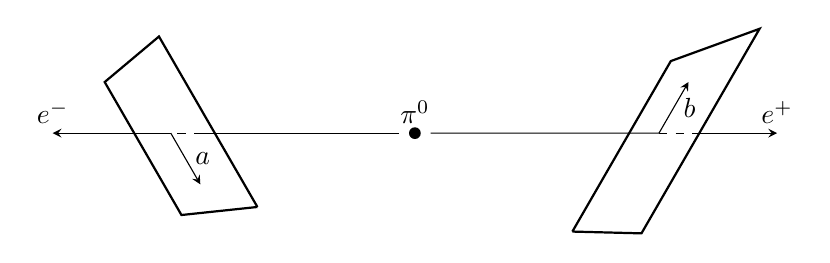
\begin{tikzpicture}
\pgfmathsetmacro{\anga}{60}
\pgfmathsetmacro{\angb}{180-\anga}
\pgfmathsetmacro{\a}{2}
\pgfmathsetmacro{\b}{1.25}
\pgfmathsetmacro{\c}{1.2}
\pgfmathsetmacro{\d}{3}
\draw[-stealth] (0.2,0) -- (3.1,0) --++ (\anga:0.75) node[pos=0.5,right]{$\kvec{b}$};
\draw[dashed](3.1,0)--++(0.5,0);
\draw[-stealth] (3.6,0) -- (4.6,0) node[above]{$e^{+}$};
\draw[] (-0.2,0) -- (-2.7,0);
\draw[dashed] (-2.7,0) -- (-3.1,0) coordinate(kl);
\draw[-stealth] (kl) --++ (\angb:-0.75) node[pos=0.5, right]{$\kvec{a}$};
\draw[-stealth] (kl) --++ (-1.5,0) node[above]{$e^{-}$};
\draw[] (0,0) node[circle, inner sep=1.5pt, fill=black]{} node[above]{$\pi^{0}$};
\draw[thick] (\a,-\b) coordinate(s) --++ (\anga:2*\b) --++ (20:\c) --++ (\anga:-\d) -- (s);
\draw[thick] (-\a,-0.75*\b) coordinate(ss) --++ (\angb:2*\b) --++ (-140:0.75*\c) --++ (\angb:-0.65*\d) -- (ss);
\end{tikzpicture}
\caption{آئنشٹائن، پوڈلسکی و  روزن  تضاد کا بل  انداز۔کاشف آزادانہ طور پر \عددی{\kvec{a}} اور \عددی{\kvec{b}} رخ سمت بند ہیں۔}
\label{شکل_بکھراو_بل_انداز}
\end{figure}


بل نے آئنشٹائن،  پوڈلسکی، روزن اور  بوہم تجربہ کو عمومی بنانے کی  تجویز پیش کی:  الیکٹران اور ضد الیکٹران کاشف کو  \ترچھا{ایک رخ}  رکھنے کی بجائے بل نے انہیں علیحدہ علیحدہ زاویوں پر رکھنے کی اجازت دی۔ پہلا کاشف اکائی سمتیہ \عددی{\kvec{a}}  کے رخ الیکٹران چکر کا جزو  ناپتا ہے،  جبکہ دوسرا \عددی{\kvec{b}}  رخ ضد الیکٹران کے چکر کا حصہ ناپتا ہے   (شکل \حوالہ{شکل_بکھراو_بل_انداز})۔ ہم اپنی آسانی کے لیے چکر کو \عددی{\hslash/2} کی اکائیوں میں ناپتے ہیں؛  یوں کاشف کے رخ ہم میدان کی قیمت \عددی{+1} اور خلاف میدان کی قیمت \عددی{-1} ناپی جائے گی۔ کئی \عددی{\pi^0} تنزل کے نتائج درج ذیل جدول میں پیش کئے گئے نتائج کی طرح ہو سکتے ہیں۔

\begin{center}
\begin{tabular}{c c c}
\toprule
الیکٹران & ضد الیکٹران &حاصل  ضرب \\
\midrule
$+1$ & $-1$ & $-1$ \\
$+1$ & $+1$ & $+1$ \\
$-1$ & $+1$ & $-1$ \\
$+1$ & $-1$ & $-1$ \\
$-1$ & $-1$ & $+1$ \\
$\vdots$ & $\vdots$ & $\vdots$ \\
\bottomrule
\end{tabular}
\end{center}

کاشف کے رخوں کی کسی ایک جوڑی کے لیے بل نے چکر کے  ترچھا{حاصل ضرب}  کی \ترچھا{ اوسط}  قیمت تلاش  کرنے کی تجویز پیش کی،  جسے ہم \عددی{P(\kvec{a},\kvec{b})} لکھتے ہیں۔ اگر کاشف متوازی ہوں،  \عددی{\kvec{b}=\kvec{a}}،  ہمیں   اصل آئنشٹائن،    پوڈلسکی،  روزن و  بوہم تشکیل  حاصل ہو گا؛  ایسی صورت میں ایک ہم میدان اور دوسرا خلاف میدان ہوگا،  لہٰذا  حاصل ضرب ہر صورت \عددی{-1} ہوگا،  اور یوں اوسط کی قیمت بھی یہی ہوگی۔
\begin{align}
	P(\kvec{a},\kvec{a}) = -1
\end{align}
اسی طرح اگر کاشف ضد متوازی ہوں، \عددی{\kvec{b}=-\kvec{a}}،  ہر حاصل ضرب \عددی{+1} ہو گا، لہٰذا درج ذیل ہوگا۔
\begin{align}
	P(\kvec{a}, -\kvec{a}) = +1
\end{align}
اختیاری سمت بندی کے لیے کوانٹائی  میکانیات درج ذیل پیشنگوئی  کرتی ہے (سوال \حوالہ{سوال_تین_اختیاری_رخ_کاشف}  دیکھیں)۔
\begin{align}
	P(\kvec{a}, \kvec{b}) = -\kvec{a}\cdot \kvec{b}
\end{align}
 بل نے دریافت کیا کہ \ترچھا{ یہ نتیجہ کسی بھی درپردہ متغیر نظریہ کا ہم آہنگ نہیں ہو سکتا}۔

اس کی دلیل حیرت کن حد تک سادہ ہے۔ فرض کریں الیکٹران و  ضد الیکٹران نظام کے \قول{ مکمل} حال کو  درپردہ متغیر (یا متغیرات)   \عددی{\lambda} ظاہر کرتا ہے۔ ( ایک پایون تنزل سے دوسرے پایون تنزل تک \عددی{\lambda} کی تبدیلی کو نہ ہم سمجھتے اور نہ ہی قابو کر سکتے ہیں۔)  ساتھ ہی فرض کریں  کہ الیکٹرانی  پیمائش پر ضد الیکٹران کاشف کی سمت بندی \عددی{\kvec{b}} کا کوئی اثر نہیں پایا جاتا؛  یاد رہے کہ تجربہ گر  الیکٹرانی پیمائش کے بعد ضد الیکٹران کاشف کا رخ منتخب کر سکتا ہے۔ ایسی صورت میں چونکہ ضد الیکٹران کاشف کا رخ منتخب کرنے سے پہلے ہی الیکٹران کی پیمائش کی جا چکی ہوگی لہٰذا اس پر \عددی{\kvec{b}}  کی  سمت کا کوئی اثر نہیں ہو سکتا۔ ( یہ اصول مقامیت کا مفروضہ ہے۔)  یوں الیکٹرانی پیمائش کوئی تفاعل \عددی{A(\kvec{a}, \lambda)} اور ضد الیکٹرانی پیمائش کوئی  دوسرا تفاعل \عددی{B(\kvec{b}, \lambda)} دیگا۔ ان تفاعلات کی قیمتیں صرف \عددی{\pm1} ہو سکتی ہیں۔
\begin{align}
	A(\kvec{a}, \lambda) = \pm1; && B(\kvec{b}, \lambda) = \pm 1
\end{align}
جب کاشف متوازی ہوں، تمام \عددی{\lambda} کے لیے  نتائج مکمل طور پر (غیر)  باہمی رشتہ :
\begin{align}\label{مساوات_پس_غیر_باہمی_رشتہ}
	A(\kvec{a}, \lambda) = -B(\kvec{a}, \lambda)
\end{align}
ہوں گے۔

 اب پیمائشوں کے  حاصل ضرب کی اوسط قیمت درج ذیل ہوگی،  جہاں \عددی{\rho(\lambda)} درپردہ متغیر کی کثافت احتمال ہے۔
\begin{align}
	P(\kvec{a}, \kvec{b}) = \int\rho(\lambda)A(\kvec{a}, \lambda)B(\kvec{b}, \lambda)\dif\lambda
\end{align}
(کسی بھی کثافت  احتمال کی طرح،  یہ غیر منفی ہوگا،  اور معمول زنی شرط \عددی{\int\rho(\lambda)\dif\lambda=1} کو مطمئن کرے گا،  لیکن  اس کے علاوہ ہم \عددی{\rho(\lambda)} کے بارے میں کچھ بھی فرض نہیں کرتے ہیں؛  درپردہ متغیر کے مختلف نظریات \عددی{\rho} کے لیے کافی مختلف تفاعلات پیش کر سکتے ہیں۔) مساوات \حوالہ{مساوات_پس_غیر_باہمی_رشتہ}    استعمال کرتے ہوئے ہم \عددی{B} کو خارج کرتے ہیں۔

%kkkk edited till here 5 march 2022

\begin{align}
	P(\kvec{a}, \kvec{b}) = -\int\rho(\lambda)A(\kvec{a}, \lambda)A(\kvec{b}, \lambda)\dif\lambda
\end{align}
اگر \عددی{\kvec{c}} کوئی تیسرا اکائی سمتیہ ہو تب درج ذیل ہوگا
\begin{align}
	P(\kvec{a}, \kvec{b})-P(\kvec{a}, \kvec{c}) = -\int\rho(\lambda)\left[A(\kvec{a}, \lambda)A(\kvec{b}, \lambda)-A(\kvec{a}, \lambda)A(\kvec{c}, \lambda)\right]\dif\lambda
\end{align}
اور چونکہ \عددی{[A(\kvec{b}, \lambda)]^2=1} ہے لہٰذا   آپ درج ذیل ہوگا 
\begin{align}
	P(\kvec{a}, \kvec{b})-P(\kvec{a}, \kvec{c}) =-\int\rho(\lambda)\left[1-A(\kvec{b}, \lambda)A(\kvec{c}, \lambda)\right]A(\kvec{a}, \lambda)A(\kvec{b}, \lambda)\dif\lambda
\end{align}
تاہم \حوالہء{مساوات \num{12.5}} کے تحت \عددی{-1\leq[A(\kvec{a}, \lambda)A(\kvec{b}, \lambda)]\leq+1} مزید \عددی{\rho(\lambda)[1-A(\kvec{b}, \lambda)A(\kvec{c}, \lambda)]\geq0} لہٰذا 
\begin{align}
	\abs{P(\kvec{a}, \kvec{b})-P(\kvec{a},\kvec{c})}\leq\int\rho(\lambda)\left[1-A(\kvec{b}, \lambda)A(\kvec{c}, \lambda)\right]\dif\lambda
\end{align}
یا مختصراً درج ذیل ہوگا
\begin{align}
	\abs{P(\kvec{a}, \kvec{b})-P(\kvec{a}, \kvec{c})}\leq1+P(\kvec{b}, \kvec{c})
\end{align}
یہ مشہور بل عدم مساوات ہے۔ \حوالہء{مساوات \num{12.5} اور \num{12.6}} کے علاوہ کوئی شرط عائد نہیں کی گئی ہے ہم نے درپردہ متغیرات کی تعداد یا خاصیت یا تقسیم \عددی{\rho} کے بارے میں کچھ بھی فرض نہیں کیا لہٰذا یہ عدم مساوات ہر مقامی درپردہ متغیر نظریہ کے لیے کارآمد ہوگا۔


\begin{figure}
\centering
\begin{tikzpicture}
\draw[-stealth] (0,0) -- (3,0) node[below]{$\kvec{a}$};
\draw[-stealth] (0,0) -- (0,3) node[left]{$\kvec{b}$};
\draw[-stealth] (0,0) --++ (45:2.5) node[above]{$\kvec{c}$};
\draw[] ([shift={(0:0.5)}]0,0) arc (0:45:0.5) node[pos=0.6,right]{$45^{o}$};
\draw[] ([shift={(45:0.75)}]0,0) arc (45:90:0.75) node[pos=0.5,shift={(67.5:0.3)}]{$45^{o}$};
\end{tikzpicture}
\caption{کاشف کو یوں سمت بند کیا گیا ہے کہ بل عدم مساوات کی کوانٹائی   خلاف ورزی   ظاہر ہو۔}
\label{شکل_بکھراو_بل_عدم_مساوات}
\end{figure}

لیکن ہم بہت آسانی سائے دکھا سکتے ہیں کہ کوانٹائی میکانیات کی پیشاً گوئی \حوالہء{مساوات \num{12.4}} اور بل عدم مساوات ہم آہنگ نہیں ہیں۔ فرض کریں تینوں اکائی سمتیات ایک مستوی میں پائے جاتے ہوں اور \عددی{a} اور \عددی{b} کے ساتھ \عددی{c} کا زاویہ \عددی{45^\circ} ہو (شکل \حوالہ{شکل_بکھراو_بل_عدم_مساوات})۔ ایسی صورت میں کوانٹائی میکانیات کہتی ہے کہ 
\begin{align*}
	P(\kvec{a}, \kvec{b}) = 0, && P(\kvec{a}, \kvec{c}) = P(\kvec{b}, \kvec{c}) = -\num{0.707}
\end{align*}
جبکہ بل عدم مساوات کہتی ہے کہ
\begin{align*}
	\num{0.707}\nleq1-\num{0.707} = \num{0.293}
\end{align*}
جو ایک دوسرے کے غیر ہم آہنگ نتائج ہیں یوں بل کی ترمیم سے آئنشٹائن، پوڈلسکی اور روزن تضاد ایک ایسی بات ثابت  کرتا ہے جو اس کے مصنفین تصور بھی نہیں کر سکتے تھے۔ اگر وہ درست ہوں تب نہ صرف کوانٹائی  میکانیات مکمل ہے بلکہ یہ مکمل طور پر غلط ہے اس کے برعکس اگر کوانٹائی میکانیات  درست ہے تب کوئی درپردہ متغیر نظریہ ہمیں اس غیر مقامیت سے نجات نہیں دو سکتی جسے آئنشٹائن مضحکہ خیز سمجھتا تھا۔	 مزید اب ہم بہت سادہ  تجربہ سے اس مسئلے کو دفنا سکتے ہیں۔

بل عدم مساوات کو پرکھنے کے لیے ساٹھ اور ستر کی دہائیوں میں کئی تجربات سرانجام دئے گئے جن میں ایسمیکٹ، گرینگیئر اور روجر کا کام قابل فخر ہے ہمیں یہاں انکے تجربہ کی تفصیل سے دلچسپی نہیں ہے۔ انہوں نے پایون تمزل کی بجائے دو نوریہ جوہری انتقال استعمال کیا یہ خدشہ دور کرنے کے لیے کہ الیکٹران کاشف کی سمت بندی کو کسی طرح ضد الیکٹران کاشف جان پائے گا  نوریہ کی روانگی کے بعد دونوں کی سمت بندی کی گئی۔نتائج کوانٹائی میکانیات کی پیشنگوئی  کی عین مطابق تھے اور بل عدم مساوات کے غیر ہم آہنگ تھے۔

ستم ظریفی کی بات ہے کہ کوانٹائی میکانیات کی تجرباتی تصدیق نے سائنسی برادری کو ہلا کر رکھ دیا۔ لیکن اس کی وجہ حقیقت پسند سوچ کا غلط ثابت ہونا نہیں تھا عموماً سائنسدان کب کے اس حقیقت کو مان چکے تھے اور جو ابھی بھی مانتے تھے انکے لیے غیر مقامی درپردہ متغیر نظریات کا راستہ ابھی کھلا ہے چونکہ مثلاً بل اطلاق ان پر نہیں ہوتا ہے۔ اصل صدمہ  اس بات کا تھا کہ قدرت خود بنیادی طور پر غیر مقامی ہے۔ تفاعل موج کی فوراً انہدام کی صورت میں غیر مقامیت یا متماثل ذرات کے لیے ضرورت تشاکلیت ہمیشہ تقلید پسند نظریہ کی خاصیت رہی ہے۔ تاہم ایسپیکٹ کے تجربہ سے قبل اُمید کی جا سکتی تھی کہ کوانٹائی غیر مقامیت کسی طرح قائد و ضوابط کی غیر طبیعی پیداوار تھی جس کے قابل کشف اثرات نہیں ہو سکتے ہیں اس اُمید کو بھول جائیں ہمیں فاصلہ پر یکدم عمل کے تصور کو دوبارہ دیکھنا ہوگا۔

\begin{figure}
\centering
\pgfmathsetmacro{\ra}{0.3}
\pgfmathsetmacro{\rb}{0.5}
\begin{tikzpicture}[declare function={fa(\t)=\ra*cos(\t); fb(\t)=\rb*sin(\t);}]
%\draw[] (0,0) circle (0.3cm and 0.5cm);
\draw[] plot[domain=120:420]({fa(\x)},{fb(\x)});
\draw[thick] ({fa(120)},{fb(120)})coordinate(bba) -- ({fa(420)},{fb(420)})coordinate(bbb)coordinate[pos=0.5](bbc);
\draw[thick](bba) to [out=90, in=90] (bbb);
\draw(bbc) to [out=90,in=45]++(0.3,0.3);
\draw(bbc) to [out=90,in=135]++(-0.3,0.3);
\draw[thin](bbc)--({fa(270)},{fb(270)});
\draw[] ({fa(35)},{fb(35)}) to [out=70,in=-160] ++ (0.2,0.2);
\draw[] ({fa(145)},{fb(145)}) to [out=110,in=-20] ++ (-0.2,0.2);
\draw[] ({fa(-45)},{fb(-45)}) to [out=-10,in=135] ++ (0.2,-0.2);
\draw[] ({fa(-135)},{fb(-135)}) to [out=-170,in=45] ++ (-0.2,-0.2);
\draw[] ({fa(0)},{fb(0)}) to [out=10,in=170] ++ (0.2,0);
\draw[] ({fa(180)},{fb(180)}) to [out=170,in=10] ++ (-0.2,0);
%
\draw[](-1,-1)--++(2,-1)node[pos=0.25,below left]{\RL{پردہ}} --++(0,4.5) --++ (-2,-0.5) -- cycle;
\draw[] (0,-1.25) node[circle, inner sep=1.5pt, fill= black]{} node[right]{$X$};
\draw[-stealth] (0,0.75) --++ (0,0.75) node[pos=0.65, right]{$\kvec{v}'$};
\draw[] (0,2) node [circle, inner sep=1.5pt, fill= black]{} node[right]{$Y$};
\draw[dashed] (-0.3,0.1) --++ (-5,0);
\draw[](-5.3,-1.3) rectangle++(-0.5,1);
\draw[thick] (-5.55,-0.3) --++ (0,0.2) coordinate(mm);
\draw[] (mm) to [out=45,in=-70] ++ (0,0.5);
\draw[] (mm) to [out=135,in=-90] ++ (0,0.5);
\fill[white] (-4.5,0.1) circle (0.3cm and 0.5cm);
\begin{scope}[xshift=-4.5cm,yshift=0.1cm, scale=0.3]
\draw[] plot[domain=120:420]({fa(\x)},{fb(\x)});
\draw[thick] ({fa(120)},{fb(120)})coordinate(bba) -- ({fa(420)},{fb(420)})coordinate(bbb)coordinate[pos=0.5](bbc);
\draw[thick](bba) to [out=90, in=90] (bbb);
\draw(bbc) to [out=90,in=45]++(0.3,0.3);
\draw(bbc) to [out=90,in=135]++(-0.3,0.3);
\draw[thin](bbc)--({fa(270)},{fb(270)});
\draw[] ({fa(35)},{fb(35)}) to [out=70,in=-160] ++ (0.2,0.2);
\draw[] ({fa(145)},{fb(145)}) to [out=110,in=-20] ++ (-0.2,0.2);
\draw[] ({fa(-45)},{fb(-45)}) to [out=-10,in=135] ++ (0.2,-0.2);
\draw[] ({fa(-135)},{fb(-135)}) to [out=-170,in=45] ++ (-0.2,-0.2);
\draw[] ({fa(0)},{fb(0)}) to [out=10,in=170] ++ (0.2,0);
\draw[] ({fa(180)},{fb(180)}) to [out=170,in=10] ++ (-0.2,0);
\end{scope}
\draw[-stealth] (-4.5,0.5) --++ (0,0.5) node[right]{$\kvec{v}$};
\draw[] (-4.5,-0.3) node[]{\RL{کیڑا}};
\end{tikzpicture}
\caption{پردہ پر کیڑے کا سایہ، روشنی کی رفتار \عددی{c} سے زیادہ رفتار \عددی{\kvec{v}'} سے  حرکت کرتا ہے بشرطیکہ  پردا  کافی دور ہو۔}
\label{شکل_بکھراو_موم_بتی}
\end{figure}

ماہر طبیعیات روشنی سے زیادہ تیز رفتار اثر و وسوخ کو کیوں برداشت نہیں کر سکتے ہیں؟ آخر کئی چیزیں روشنی سے زیادہ تیز رفتار سے حرکت کرتی ہے۔ ایک موم بتی کے سامنے چلتے ہوئے کیڑے کا سامنے دیوار پر سائے  کی رفتار دیوار تک فاصلے کے راست متناسب ہوگی اصولاً آپ اس فاصلہ کو اتنا بڑھا سکتے ہیں کہ سایہ کی رفتار روشنی سے زیادہ ہو (شکل \حوالہ{شکل_بکھراو_موم_بتی})۔ تاہم دیوار پر کسی ایک نقطہ سے دوسرے نقطہ تک سایہ نہ کوئی توانائی منتقل کر سکتا ہے اور نہ ہی کوئی خبر پہنچا سکتا ہے۔ نقطہ \عددی{X} پر ایک شخص ایسا کوئی عمل نہیں کر سکتا جو یہاں سے گزرتے ہوئے سائے کے ذریعہ نقطہ \عددی{Y} پر اثر انداز ہو۔

%===============================

اس کے برعکس روشنی سے زیادہ تیز حرکت کرنے والے سببی اثر و وسوخ کے ناقابل قبول مضمرات ہو سکتے ہیں۔ خصوصی نظریہ اضافت میں ایسے جمودی چوکھٹ پائے جاتے ہیں جن میں اس طرح کا اشارہ وقت میں پیچھے جا سکے گا یعنی سبب سے پہلے اثر رونما ہوگا جس سے ناقابل قبول منتقی  مسائل کھڑے ہوتے ہیں۔ مثلاً آپ اپنے نوزائیدہ   دادا کو قتل کر سکتے ہیں۔ جو ظاہر ہے ایک بری بات ہے۔ اب سوال یہ کھڑا ہوتا ہے کہ آیا روشنی سے تیز اثرات جن کی پیشنگوئی  کوانٹائی میکانیات کرتی ہے اور جو ایسپیکٹ کے تجربہ میں کسف ہعتے ہیں ان معنوں میں سببی ہے یا یہ سائے کی حرکت کی طرح غیر حقیقی ہے جن پر فلسفیانہ  اعتراضات نہیں لگائے جا سکتے ہیں۔

آئیں تجربہ بل پر غور کریں کریں۔ کیا الیکٹران کی پیمائش کا ضد الیکٹران کی پیمائش پر اثر ہوگا  یقیناً ایسا ہوتا ہے ورنہ ہم مواد کے بیچ باہم رشتہ کی وضاحت پیش کرنے سائے قاصر ہوں گے۔ لیکن کیا الیکٹران کی پیمائش ضد الیکٹران کی کسی مخصوص نتیجہ کا سبب ہے؟ الیکٹران کاشف پر بیٹھا  شخص اپنی پیمائش کے ذریعہ ضد الیکٹران کاشف پر بیٹھے شخص کو اشارہ نہیں بھیج سکتا ہے چونکہ یہ اپنی پیمائش کے نتیجہ کو قابو نہیں کرتا یہ الیکٹران کو ہم میدان ہونے پر مجبور نہیں  کر سکتا ہے جیسا نقطہ \عددی{X} پر کیڑا کے سائے پر وہ شخص اثر انداز نہیں ہو سکتا، ہاں الیکٹران کاشف پر بیٹھا شخص فیصلہ کر سکتا ہے کہ وہ پیمائش کرے یا نہ کرے تاہم ضد الیکٹران کاشف پر بیٹھا شخص اپنی پیمائشی نتائج کو دیکھ کر یہ نہیں بتا سکتا کہ الیکٹران پر پیمائش کی گئی یا نہیں دونوں کاشف کے نتائج پر علیحدہ علیحدہ غور کرنے سے مکمل بلا واسطہ مواد دیکھنے کو ملتا ہے۔ صرف دونوں مواد کا ایک دوسرے کے ساتھ موازنہ کرنے سے ہمیں ان کے بیچ باہم رشتہ نظر آتا ہے کسی دوسرے جمودی چوکھٹ میں الیکٹران کی پیمائش سے قبل ضد الیکٹران کی پیمائش کی جائے گی لیکن اس کے باوجود اس سے کوئی منتقی تضاد پیدا نہیں ہوتا۔ دکھا گیا باہم رشتہ اس پر منحصر نہیں کہ ہم کہیں الیکٹران کی پیمائش ضد الیکٹران کی پیمائش پر اثر انداز ہوتی ہے یا ضد الیکٹران کی پیمائش الیکٹران کی پیمائش پر اثر انداز ہوتی ہے۔ یہ ایک نہایت نازک اور خوبصورت اثر ہے جو بلا واسطہ مواد کے بیچ باہم رشتہ کی صورت میں نظر آتا ہے۔

یوں ہمیں مختلف قسم کے اثرات کی بات کرنی ہوگی سببی قسم جو وصول کنندہ کی کسی طبیعی خاصیت میں حقیقی تبدیلیاں پیدا کرتا ہو جنہیں صرف ذیلی نظام پر تجرباتی پیمائش سے کشف کیا جا سکتا ہو اور آسمانی  قسمپ جو توانائی یا معلومات کی ترسیل نہیں کرتا اور جس کے لیے واحد ثبوت دو علیحدہ ذیلی نظاموں کے مواد کے بیچ باہم رشتہ ہے۔ اس باہم رشتہ کو کسی بھی طرح کسی ایک ذیلی نظام میں تجربات کے نتائج کو دیکھ کر کشف نہیں کیا جا سکتا ہے۔ سببی اثرات  روشنی کی رفتار سے تیز حرکت نہیں کر سکتے ہیں جبکہ آسمانی  اثرات پر ایسی کوئی پابندی عائد نہیں۔ تفاعل موج کی انہدام سے وابستہ اثرات موخر الذکر قسم کی ہے جس کا روشنی سے تیز سفر کرنا حیران کن ضرور ہو سکتا ہے لیکن تباہ کن نہیں ہے۔
%========================

\حصہ{مسئلہ کلمیہ}
کوانٹائی پیمائش عموماً تباہ کن ہوتے ہیں یعنی یہ پیمائش کردہ نظام کے حال کو تبدیل کرتا ہے۔ یہی تجربہ گاہ میں اصول عدم یقینیت کو یقینی بناتا ہے ہم کیوں اصل حال کی کئی متماثل نقل کلمیہ بنا کر اصل نظام کو چھوئے بغیر ان کی پیمائش نہیں کرتے ایسا کرنا ممکن نہیں ہے۔ اگر آپ کلمیہ بنانے والا ایسا آلا بنا پائیں تو کوانٹائی میکانیات کو خدا حافظ کہنا ہوگا۔

مثال کے طور پر آئنشٹائن، پوڈلسکی، روزن اور بوہم تجربہ کے ذریعہ روشنی سے تیز رفتار پر خبر بھیجنا ممکن ہوگا فرض کریں ضد الیکٹران کاشف چلانے والا شخص ہاں یا نہیں کی خبر ترسیل کرتا ہے۔ خبر ہاں ہونے کی صورت میں بھیجنے والا ضد الیکٹران کا \عددی{S_z} ناپتا ہے یہ جاننے کی ضرورت نہیں کہ پیمائشی نتیجہ کیا ہے صرف اتنا جاننا ضروری ہے کہ پیمائش کی گئی ہے یوں الیکٹران کسی غیر مبہم حال \عددی{\uparrow} یا \عددی{\downarrow} میں ہوگا جس کا جاننا غیر اہم ہے۔ خبر وصول کرنے والا جلدی سے الیکٹران کی دس لاکھ کلمیہ تیار کر کے ہر ایک کی \عددی{S_z} ناپتا ہے اگر تمام کا ایک ہی جواب ہو کونسا جواب یہ جاننا ضروری نہیں ہم یقین سے کہہ سکیں گے کہ الیکٹران کی پیمائش کی گئی لہٰذا خبر ہاں ہوگی۔ اس کے برعکس اگر نصف الیکٹران ہم میدان اور نصف خلاف میدان ہوں تب یقیناً الیکٹران کی پیمائش نہیں کی گئی اور خبر نہیں ہوگا۔

لیکن سن \num{1982} ووٹرز، زورک اور ڈائکس نے ثابت کیا کہ ایسا مشین تیار نہیں کیا جا سکتا ہے جو کوانٹائی متماثل ذرات پیدا کرتا ہو ہم چاہیں گے کہ یہ مشین حال \عددی{|\psi\rangle} میں ایک ذرہ جس کا نقل بنانا مقصود ہو اور حال \عددی{| X\rangle} میں ایک اضافی ذرہ لی کر  حال \عددی{|\psi\rangle} میں دو ذرات  اصل اور نقل دیتا ہو 
\begin{align}
	|\psi\rangle| X\rangle\to|\psi\rangle|\psi\rangle
\end{align}
فرض کریں ہم ایسا مشین بنانے میں کامیاب ہوتے ہیں جو حال \عددی{|\psi_1\rangle} کا کلمہ تیار کرتا ہو 
\begin{align}
	|\psi_1\rangle| X\rangle\to|\psi_1\rangle|\psi_1\rangle
\end{align}
اور \عددی{|\psi_2\rangle} پر بھی کام کرنے کے قابل ہو
\begin{align}
	|\psi_2\rangle| X\rangle\to|\psi_2\rangle|\psi_2\rangle
\end{align}
مثال کے طور پر اگر ذرہ ایک الیکٹران ہو تب \عددی{|\psi_1\rangle} اور \عددی{|\psi_2\rangle} ہم میدان اور خلاف میدان ہو سکتے ہیں۔ یہاں تک کوئی مسئلہ پیدا نہیں ہوتا یہ دکھانا ہوگا کہ ان کا خطی جوڑ \عددی{|\psi\rangle=\alpha|\psi_1\rangle+\beta|\psi_2\rangle} کی صورت میں کیا ہوگا؟ ظاہر ہے ایسی صورت میں درج ذیل ہوگا
\begin{align}
	|\psi\rangle| X\rangle\to\alpha|\psi_1\rangle|\psi_1\rangle+\beta|\psi_2\rangle|\psi_2\rangle
\end{align}
جو ہم نہیں چاہتے ہیں۔ ہم درج ذیل چاہتے ہیں  
\begin{align}
	|\psi\rangle| X\rangle\to|\psi\rangle|\psi\rangle &= [\alpha|\psi_1\rangle+\beta|\psi_2\rangle][\alpha|\psi_1\rangle+\beta|\psi_2\rangle]\nonumber \\
	&= \alpha^2|\psi_1\rangle|\psi_1\rangle+\beta^2|\psi_2\rangle|\psi_2\rangle+\alpha\beta[|\psi_1\rangle|\psi_2\rangle+|\psi_2\rangle|\psi_1\rangle]
\end{align}
آپ ہم میدان الیکٹران اور خلاف میدان الیکٹران کے کلمہ بنانے کی مشین بنا سکتے ہیں لیکن وہ کسی بھی با وقعت (غیر صفر)  خطی جوڑ کی صورت میں ناکامی کا شکار ہوگا یہ بالکل ایسا ہوگا جیسا نقل بنانے کی مشین  افقی لکیروں اور انتصابی لکیروں کی نقل خوش اسلوبی سے کرتا ہو لیکن وتری لکیروں کو مکمل طور پر بگاڑتا ہو۔
%================

\حصہ{شروڈنگر کی بلی}
کوانٹائی میکانیات میں پیمائش کا عمل ایک شرارتی کردار ادا کرتا ہے جس میں عدم تعینیت غیر مقامیت تفاعل موج کا انہدام اور باقی تمام تصوراتی مشکلات رونما ہوتی ہیں۔ پیمائش کی غیر موجودگی میں مساوات شروڈنگر کے تحت تفاعل موج قابل تعین طریقہ سے ارتقا کرتا ہے اور کوانٹائی میکانیات کسی بھی سادہ نظریہ میدان کی طرح نظر آتا ہے جو کلاسیکی برقی حرکیات سے بہت سادہ ہوگا چونکہ دو میدان \عددی{E} اور \عددی{B} کی بجائے اس میں واحد ایک غیر سمتی \عددی{\psi} پایا جاتا ہے۔ یہ پیمائش کا عمل ہی ہے جو کوانٹائی میکانیات میں عجیب و غریب کردار ادا کرتے ہوئے اس کو سمجھ سے باہر خواص سے نوازتا ہے۔ یہ پیمائش حقیقت میں ہے کیا؟ اسے گیگر طبیعی عوامل سے کیا منفرد بناتا ہے اور ہم کس طرح جان سکتے ہیں کہ پیمائش کی گئی ہے؟

شروڈنگر نے اپنے مشہور تضاد  ب بلی کے مفروضہ نے اس بنیادی سوال کو پیش کیا۔

ایک بلی کو فولاد کے ایک بند ڈبے میں بند کیا جاتا ہے اس ڈبے میں ایک گائگر  گنت کار اور کسی تابکار مادہ کی اتنی چھوٹی مقدار رکھی جاتی ہے جس کا ایک گھنٹہ  میں صرف ایک جوہر کے تنزل  کا امکان ہو تاہم یہ بھی ممکن ہے کہ کوئی جوہر تنزل  نہ ہو تنزل  کی صورت میں گنت کار اس ڈبے میں ایک زہریلی گیس چھوڑتا ہے۔ ایک گھنٹہ گزرنے کے بعد ہم کہہ سکتے ہیں کہ تنزل نہ ہونے کی صورت میں یہ بلی زندہ ہوگی۔ پہلا  تنزل  اس کو زہر سے مار دیتی۔اس مکمل نظام کا تفاعل موج اس حقیقت کو ظاہر کرنے کے لیے زندہ اور مردہ بلی کے برابر حصوں پر مشتمل ہوگا۔

ایک گھنٹہ کے بعد بلی کا تفاعل موج درج ذیل روپ کا ہوگا
\begin{align}
	\psi=\frac{1}{\sqrt{2}}(\psi_{\text{\RL{زندہ}}}+\psi_{\text{\RL{مردہ}}})
\end{align}
یہ بلی نہ تو زندہ اور نہ ہی مردہ ہے بلکہ پیمائش سے پہلے یہ ان دونوں کا ایک خطی جوڑ ہوگا یہاں کھڑکی سے اندر دیکھ کر بلی کا حال جاننے کو پیمائش تصور کیا جائے گا۔ آپ کا دیکھنے کا عمل بلی کو زندہ یا مردہ ہونے پر مجبور کرتا ہے ایسی صورت میں اگر بلی مردہ پائی جائے تو یقیناً اس کے ذمہ دار آپ ہی ہیں چونکہ آپ نے کھڑکی سے دیکھ کر اسے قتل کیا۔

شروڈنگر اس تمام کو ایک بکواس سے زیادہ نہیں سمجھتا تھا اور میرے خیال سے زیادہ تر ماہر طبیعیات ان  کے ساتھ متفق ہیں۔ کلاں بین اجسام کا دو مختلف حالات کی ایک خطی جوڑ کی صورت میں ہونے کا تصور بے معنی ہے۔ ایک الیکٹران تو ہم میدان اور خلاف میدان کے ایک خطی جوڑ کی صورت میں ہو سکتا ہے لیکن ایک بلی زندہ اور مردہ حالات کے ایک خطی جوڑ کی صورت میں نہیں ہو سکتی ہے۔ اس کو کوانٹائی میکانیات کی تقلید پسند تشریح کے ساتھ کس طرح ہم آہنگ بنایا جا سکتا ہے۔

شماریاتی مفہوم کے لحاظ سے مقبول ترین جواب یہ ہے کہ گنت کار کی گنتی پیمائش ہوگی نہ کہ کھڑکی میں سے انسانی مشاہدہ پیمائش سے مراد وہ عمل ہے جو کلاں بین نظام پر اثر انداز ہو جو یہاں گنت کار ہے۔ پیمائش کا عمل اس لمحہ پر رونما ہوگا جب خوردبین نظام جسے کوانٹائی میکانیات کے قوانین بیان کرتا ہے کلاں بین نظام جسے کلاسیکی میکانیات کے قواعد بیان کرتے ہیں کے ساتھ اس طرح باہم عمل کرے جس سے دائمی تبدیلی رونما ہو۔ کلاں بین نظام خود منفرد حالات کی ایک خطی جوڑ کا مکین نہیں ہو سکتا ہے۔

\حصہ{کوانٹائی زینو تضاد}
اس عجیب قصہ کی اہم ترین خاصیت تفاعل موج کا انہدام ہے۔ ایک پیمائش کے فوراً بعد دوسری پیمائش سے اسی نتیجہ کے حصول کی خاطر خالصتاً نظریاتی بنیادوں پر اسے متعارف کیا گیا تھا یقیناً اس دو رس  اصول موضوعہ کے قابل مشاہدہ اثرات بھی ہوں گے۔ مسرا اور سدرشان نے سن \num{1977} میں تفاعلی موج کی انہدام کا ایک ڈرامائی تجرباتی مظاہرہ تجویز کیا جسے انہوں نے کوانٹائی زینو اثر کا نام دیا۔ ان کا تصور یہ تھا کہ ایک غیر مستحکم نظام مثلاً ہیجان حال میں ایک جوہر کو بار بار پیمائشی عمل سے گزارا جائے۔ ہر ایک مشاہدہ تفاعل موج کو منہدم کر کے گھڑی کو دوبارہ صفر  سے چالو کرے گا اور یوں زیریں حال میں متوقع  انتقال کو غیر معائنہ مدد تک روکا جا سکتا ہے۔

فرض کریں ایک نظام ہیجان حال \عددی{\psi_2} سے آغاز کرتا ہے اور زمینی حال \عددی{\psi_1} میں منتقلی کے لیے اس کا قدرتی عرصہ حیات \عددی{\tau} ہے۔ عام طور پر \عددی{\tau} سے کافی کم وقتوں کے لیے انتقالی احتمال وقت \عددی{t} کا راست متناسب ہوگا \حوالہء{مساوات \num{9.42}} دیکھیں چونکہ انتقالی شرح \عددی{1/\tau} ہے لہٰذا درج ذیل ہوگا 
\begin{align}
	P_{2\to1}=\frac{t}{\tau}
\end{align}
وقت \عددی{t} پر پیمائش کرنے کی صورت میں بالائی حال میں نظام ہونے کا احتمال درج ذیل ہوگا
\begin{align}
	P_2(t)=1-\frac{t}{\tau}
\end{align}
فرض کریں ہم دیکھتے ہیں کے نظام بالائی حال میں ہی ہے ایسی صورت میں تفاعل موج واپس \عددی{\psi_2} پر منہدم ہوگا اور پورا عمل ایک بار نئے سرے سے دوبارہ شروع ہوگا۔ اگر ہم وقت \عددی{2t} پر دوسری پیمائش کریں تب بالائی حال میں نظام ہونے کا احتمال درج ذیل ہوگا 
\begin{align}
	\left(1-\frac{t}{\tau}\right)^2\approx1-\frac{2t}{\tau}
\end{align}
جو وہی ہے جو اس صورت ہوتا اگر ہم پہلی پیمائش کرتے ہی نہیں سادہ سوچ کے تحت ایسا ہی ہونا چاہیے  تھا۔ اگر ایسا ہی ہوتا تب نظام کا بار بار مشاہدہ کرنے سے کوئی فرق نہیں پڑتا اور نہ یہ  کوانٹائی زینو اثر پیدا ہوتا تاہم بہت کم وقت کی صورت میں انتقالی احتمال وقت \عددی{t} کے بجائے \عددی{t^2} کا راست متناسب ہوگا \حوالہء{\num{9.39}} دیکھیں
\begin{align}
	P_{2\to1}=\alpha t^2
\end{align}
ایسی صورت میں دو پیمائشوں کے بعد بھی نظام کا بالائی حال میں ہونے کا احتمال درج ذیل ہوگا
\begin{align}
	\left(1-\alpha t^2\right)^2\approx 1-2\alpha t^2
\end{align}
جبکہ پہلی پیمائش نہ کرنے کی صورت میں اب احتمال درج ذیل ہوتا
\begin{align}
	1-\alpha(2t)^2\approx1-4\alpha t^2
\end{align}
آپ دیکھ سکتے ہیں کہ وقت \عددی{t} گزرنے کے بعد نظام کے مشاہدہ کی بنا پر زیریں حال میں منتقلی کا احتمال کم ہوا ہے۔

یقیناً \عددی{t=0} سے لیکر \عددی{t=T} تک \عددی{n} برابر وقفہ \عددی{T/n, 2T/n, 3T/n, \dots, T} پر نظام کا مشاہدہ کرنے کی وجہ سے اس دورانیہ کے آخر میں بھی نظام بالائی حال میں پائے جانے کا احتمال درج ذیل ہوگا
\begin{align}
	\left(1-\alpha(T/n)^2\right)^n\approx1-\frac{\alpha}{n}T^2
\end{align}
جو \عددی{n\to\infty} کی حد میں \عددی{1} تک پہنچتا ہے ایک غیر مستحکم نظام جس کا مسلسل مشاہدہ کیا جائے کبھی بھی تحویل نہیں ہوگا بعض مصنفین اس ماخوذ  سے اتفاق نہیں کرتے اور ان کے نزدیک یہ تفاعل موج کے انہدام غیر درست ہونے کا ثبوت ہے۔ تاہم ان کے دلائل مشاہدہ کے مفہوم کی غلط تشریح پر مبنی ہے اگر بلبلا خانہ میں ایک ذرہ کی راہ کو مسلسل مشاہدہ قرار دے دیا جائے تب یہ بالکل درست ہوں گے چونکہ ایسی ذرات یقیناً تحویل ہوتے ہیں اور ان کا عرصہ حیات پر کاشف کا قابل پیمائش اثر نہیں پایا جاتا ہے تاہم ایسا ذرہ خانہ کے اندر جوہروں کے ساتھ خدوخال  باہم عمل کرتا ہے جبکہ کوانٹائی زینو اثر کے لیے ضروری ہے کہ یک بعد دیگر پیمائشوں کے بیچ وقفہ اتنا کم ہو کہ نظام کو \عددی{t^2} خطہ میں پکڑا جائے۔

ہم دیکھتے ہیں کہ خود با خود انتقل کی صورت میں یہ تجربہ عملاً ممکن نہیں ہے۔ تاہم پیدا کردہ انتقال کی صورت میں نتائج کا نظریاتی پیشنگوئی کے ساتھ مکمل اتفاق پایا جات ہے۔ بدقسمتی سے یہ تجربہ تفاعل موج کی انہدام کا  حتمی  ثبوت پیش نہیں کر سکتا ہے اس مشاہدہ کے دیگر وجوہات بھی دئے جا سکتے ہیں۔ 

میں نے اس کتاب میں ایک ہم آہنگ  اور بلا تضاد کہانی پیش کرنے کی کوشش کی ہے تفاعل موج \عددی{\psi} کسی ذرہ یا نظام کے حال کو ظاہر کرتا ہے۔ عمومی طور پر ای کذرہ کسی مخصوص حرکی خاصیت مثلاً مقام معیار حرکت توانائی زاویائی معیار حرکت وغیرہ کا حامل نہیں ہوتا اس وقت تک  جب پیمائشی عمل مداخلت نہ کرے کسی ایک تجربہ میں حاصل ایک مخصوص قیمت کا احتمال \عددی{\psi} کی شماریاتی مفہوم تعین کرتا ہے۔ پیمائشی عمل سے تفاعل موج منہدم ہوتا ہے جس کی بنا پر فوراً دوسری پیمائش لازماً وہی نتیجہ دیگی۔ اگرچہ دیگر تشریحات مثلاً غیر مقامی درپردہ متغیر نظریات متعدد کائنات کا تصور بلا تضاد تاریخیں  سگرہ نمونے وغیرہ بھی پائے جاتے ہیں لیکن میں یقین کرتا ہوں کہ یہ سب سے سادہ ہے جس سے عموماً ماہر طبیعیات اتفاق کرتے ہیں۔ یہ ہر تجربہ سے کامیابی سے ابھرا ہے تاہم یہ کہانی کا اختتام نہیں ہے ہمیں پیمائشی عمل کے بارے میں اور انہدام کے طریقے کار کے بارے میں بہت کچھ جاننا ہے عین ممکن ہے کہ آنے والے نسلیں زیادہ پیچیدہ  نظریہ جانتے ہوئے سوچتے ہوں کہ ہم اتنا سادہ کیسے ہو سکتے تھے۔

